\begin{activity} \label{A:5.2.2}  Suppose that $f(t) = \frac{t}{1+t^2}$ and $F(x) = \int_0^x f(t) \, dt$.

\begin{figure}[h]
\begin{center}

\includegraphics{figures/5_2_Act2.eps}
\end{center}
\caption{Axes for plotting $f$ and $F$.} \label{F:5.2.Act2}
\end{figure}
\ba
	\item On the axes at left in Figure~\ref{F:5.2.Act2}, plot a graph of $f(t) = \frac{t}{1+t^2}$ on the interval $-10 \le t \le 10$.  Clearly label the vertical axes with appropriate scale.
	\item What is the key relationship between $F$ and $f$, according to the Second FTC?
	\item Use the first derivative test to determine the intervals on which $F$ is increasing and decreasing.
	\item Use the second derivative test to determine the intervals on which $F$ is concave up and concave down.  Note that $f'(t)$ can be simplified to be written in the form $f'(t) = \frac{1-t^2}{(1+t^2)^2}.$
	\item Using technology appropriately, estimate the values of $F(5)$ and $F(10)$ through appropriate Riemann sums.
	\item Sketch an accurate graph of $y = F(x)$ on the righthand axes provided, and clearly label the vertical axes with appropriate scale.
\ea
\end{activity}
\begin{smallhint}
\ba
	\item Use computing technology appropriately to generate the desired graph.
	\item Again, recall the statement of the Second FTC.
	\item Where is $F'$ positive?  $F'$ negative?
	\item Note that $F'' = f'$.
	\item Remember that $F(5) = \int_0^5 \frac{t}{1+t^2} \, dt$.
	\item Don't forget that $F(0) = 0$.
\ea
\end{smallhint}
\begin{bighint}
\ba
	\item Use computing technology appropriately to generate the desired graph.
	\item Again, recall the statement of the Second FTC.
	\item Where is $F'$ positive?  $F'$ negative?  Remember that $F$ is increasing wherever $F'$ is positive.
	\item Note that $F'' = f'$, which tells us that $F''(t) = \frac{1-t^2}{(1+t^2)^2}$.  Where is $F''$ positive? negative?
	\item Remember that $F(5) = \int_0^5 \frac{t}{1+t^2} \, dt$.  Try a midpoint sum with at least 10 subintervals.
	\item Don't forget that $F(0) = 0$.  Use the values and information you've found in (b)-(e).
\ea
\end{bighint}
\begin{activitySolution}
\ba
	\item See the plot at below left.
	\item $F' = f$, by the Second FTC.
	\item $F$ is increasing wherever $F'=f$ is positive, so for all $x > 0$.  Similarly, $F$ is decreasing for $x < 0$
	\item $F$ is CCU wherever $F' = f$ is increasing or wherever $F'' = f'$ is positive.  It is straightforward to show that $f''$ is positive for $-1 < x < 1$ and negative otherwise, thus $F$ is CCU on $-1 < x < 1$ and CCD for $x < -1$ and $x > 1$.
	\item $F(5) = \int_0^5 \frac{t}{1+t^2} \, dt \approx 2.35973$, using a midpoint Riemann sum with 10 subintervals.  Similarly, $F(10) = \int_0^{10} \frac{t}{1+t^2} \, dt \approx 2.35973$.
	\item Recalling that $F(0) = 0$ and using the values and information we've found in (b)-(e), we arrive at the graph at below right.
\ea
\begin{center}
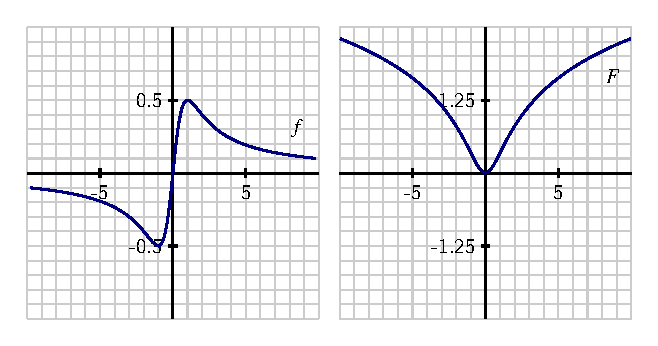
\includegraphics{figures/5_2_Act2_soln.eps}
\end{center}
\end{activitySolution}
\aftera